%% LyX 2.3.4.2 created this file.  For more info, see http://www.lyx.org/.
%% Do not edit unless you really know what you are doing.
\documentclass[11pt,english]{article}
\usepackage{mathpazo}
\usepackage[T1]{fontenc}
\usepackage[utf8]{inputenc}
\usepackage[paperwidth=6in,paperheight=9in]{geometry}
\geometry{verbose,tmargin=0.8in,bmargin=0.7in,lmargin=0.75in,rmargin=0.5in}
\setcounter{secnumdepth}{-2}
\setcounter{tocdepth}{-2}
\setlength{\parskip}{\medskipamount}
\setlength{\parindent}{0pt}
\usepackage[active]{srcltx}
\usepackage{color}
\usepackage{babel}
\usepackage{float}
\usepackage{graphicx}
\usepackage[unicode=true,pdfusetitle,
 bookmarks=true,bookmarksnumbered=false,bookmarksopen=false,
 breaklinks=true,pdfborder={0 0 0},pdfborderstyle={},backref=false,colorlinks=true]
 {hyperref}
\hypersetup{
 urlcolor=blue, linkcolor=blue, citecolor=blue}

\makeatletter
%%%%%%%%%%%%%%%%%%%%%%%%%%%%%% User specified LaTeX commands.
\usepackage{cite}
\usepackage[margin=10pt,font=small,labelfont=bf]{caption}
\usepackage[all]{hypcap}  % links to top of Figure s

\makeatother

\begin{document}

\subsection{Project Title}

Team Members: (List the project participants here)

\subsubsection{Summary}

Background describing what the purpose for which the material is being designed. This is basically a description of the performance characteristics of the material. Add references using the format shown here for this example reference \cite{rondinelli_accelerating_nodate}.

\subsubsection{System Design Chart}

Include your system design chart here, with a description of the relationships between the different elements. The composites design chart is included as an example here. Put the system chart in a figure float, like the one shown here as Figure \ref{fig:system chart}, and refer to it
as done in this example.

\begin{figure}[H]
\begin{centering}
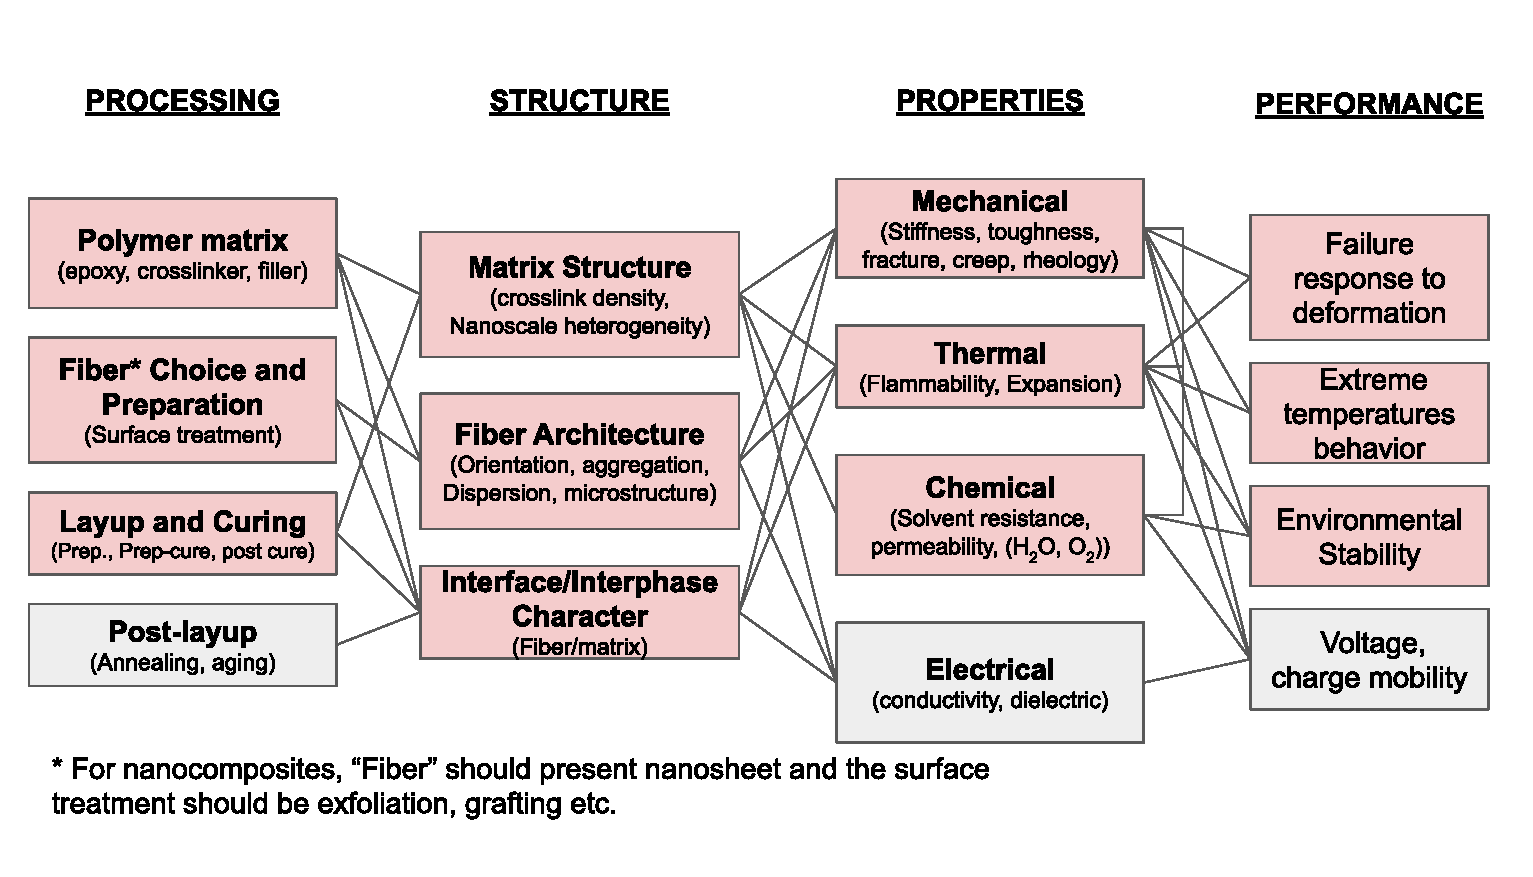
\includegraphics[width=1\textwidth]{system_chart_example}
\par\end{centering}
\caption{Figure Caption Here\label{fig:system chart}}

\end{figure}


\subsubsection{Materials Selection}

Use the CES Materials Selector software to describe how the generic material you choose to investigate is the right material to meet the performance characteristics specified in your design chart.

\subsubsection{Design Strategy}

Describe your overall the design strategy for a new or enhanced material, describing how different elements in the system design chart will be addressed. For the purposes of 390, assume that you had full quarter to address the problem, with access to an experimental lab. Describe one particular aspect of the design process that you will address with computational tools. 

\subsubsection{Results}

Given the constraints of the 2020 spring quarter, results are obviously going to limited. In light of this, due your best to use computational tools (most likely COMSOL or ThermoCalc to improve your design in one specific area.

\bibliographystyle{MSEcore}
\bibliography{390}

\end{document}
